\documentclass[conference]{IEEEtran}
\IEEEoverridecommandlockouts
\usepackage{cite}
\usepackage{amsmath,amssymb,amsfonts}
\usepackage{graphicx}
\usepackage{textcomp}
\usepackage{xcolor}
\usepackage{booktabs}
\usepackage{braket}
% auto-generated by project/scripts/make_paper_assets.py
\newcommand{\Nrows}{40{,}564}
\newcommand{\Npool}{25{,}318}
\newcommand{\Ntest}{15{,}246}
\newcommand{\Nused}{2{,}000}
\newcommand{\Thr}{3340}
\newcommand{\accOursC}{0.912}
\newcommand{\sdOursC}{0.022}
\newcommand{\accOursD}{0.942}
\newcommand{\sdOursD}{0.006}
\newcommand{\accOursM}{0.947}
\newcommand{\sdOursM}{0.001}
\newcommand{\accOursMM}{0.949}
\newcommand{\sdOursMM}{0.003}
\newcommand{\aucOurs}{0.980}
\newcommand{\foneOurs}{0.950}
\newcommand{\recOurs}{0.929}
\newcommand{\fitOurs}{5.3}
\newcommand{\accStdC}{0.913}
\newcommand{\sdStdC}{0.010}
\newcommand{\accStdD}{0.917}
\newcommand{\sdStdD}{0.007}
\newcommand{\accStdM}{0.910}
\newcommand{\sdStdM}{0.002}
\newcommand{\accStdMM}{0.906}
\newcommand{\sdStdMM}{0.005}
\newcommand{\aucStd}{0.971}
\newcommand{\foneStd}{0.913}
\newcommand{\recStd}{0.890}
\newcommand{\fitStd}{2.3}
\newcommand{\accQKC}{0.710}
\newcommand{\sdQKC}{0.031}
\newcommand{\accQKD}{0.844}
\newcommand{\sdQKD}{0.010}
\newcommand{\accQKM}{0.865}
\newcommand{\sdQKM}{0.002}
\newcommand{\accQKMM}{0.870}
\newcommand{\sdQKMM}{0.002}
\newcommand{\aucQK}{0.926}
\newcommand{\foneQK}{0.872}
\newcommand{\recQK}{0.856}
\newcommand{\fitQK}{6.3}
\newcommand{\accLRC}{0.919}
\newcommand{\sdLRC}{0.003}
\newcommand{\accLRD}{0.924}
\newcommand{\sdLRD}{0.002}
\newcommand{\accLRM}{0.917}
\newcommand{\sdLRM}{0.006}
\newcommand{\accLRMM}{0.921}
\newcommand{\sdLRMM}{0.005}
\newcommand{\aucLR}{0.972}
\newcommand{\foneLR}{0.921}
\newcommand{\recLR}{0.900}
\newcommand{\fitLR}{0.0}
\newcommand{\accSVMC}{0.925}
\newcommand{\sdSVMC}{0.001}
\newcommand{\accSVMD}{0.942}
\newcommand{\sdSVMD}{0.002}
\newcommand{\accSVMM}{0.944}
\newcommand{\sdSVMM}{0.002}
\newcommand{\accSVMMM}{0.946}
\newcommand{\sdSVMMM}{0.003}
\newcommand{\aucSVM}{0.980}
\newcommand{\foneSVM}{0.947}
\newcommand{\recSVM}{0.926}
\newcommand{\fitSVM}{0.1}
\newcommand{\accRFC}{0.930}
\newcommand{\sdRFC}{0.007}
\newcommand{\accRFD}{0.941}
\newcommand{\sdRFD}{0.007}
\newcommand{\accRFM}{0.938}
\newcommand{\sdRFM}{0.004}
\newcommand{\accRFMM}{0.939}
\newcommand{\sdRFMM}{0.002}
\newcommand{\aucRF}{0.980}
\newcommand{\foneRF}{0.941}
\newcommand{\recRF}{0.918}
\newcommand{\fitRF}{0.4}
\newcommand{\accMLPC}{0.918}
\newcommand{\sdMLPC}{0.017}
\newcommand{\accMLPD}{0.947}
\newcommand{\sdMLPD}{0.001}
\newcommand{\accMLPM}{0.945}
\newcommand{\sdMLPM}{0.003}
\newcommand{\accMLPMM}{0.949}
\newcommand{\sdMLPMM}{0.001}
\newcommand{\aucMLP}{0.983}
\newcommand{\foneMLP}{0.947}
\newcommand{\recMLP}{0.927}
\newcommand{\fitMLP}{1.0}
\newcommand{\accOursFifty}{0.814}
\newcommand{\ablA}{0.917}
\newcommand{\ablAsd}{0.007}
\newcommand{\ablAp}{26}
\newcommand{\ablB}{0.896}
\newcommand{\ablBsd}{0.012}
\newcommand{\ablBp}{26}
\newcommand{\ablC}{0.942}
\newcommand{\ablCsd}{0.006}
\newcommand{\ablCp}{50}
\newcommand{\ablD}{0.918}
\newcommand{\ablDsd}{0.009}
\newcommand{\ablDp}{38}
\newcommand{\ablE}{0.944}
\newcommand{\ablEsd}{0.005}
\newcommand{\ablEp}{50}
\newcommand{\ablF}{0.772}
\newcommand{\ablFsd}{0.088}
\newcommand{\ablFp}{50}
\newcommand{\ablG}{0.559}
\newcommand{\ablGsd}{0.017}
\newcommand{\ablGp}{18}
\newcommand{\ablH}{0.939}
\newcommand{\ablHsd}{0.011}
\newcommand{\ablHp}{34}
\newcommand{\ablI}{0.939}
\newcommand{\ablIsd}{0.002}
\newcommand{\ablIp}{66}
\newcommand{\ablJ}{0.942}
\newcommand{\ablJsd}{0.005}
\newcommand{\ablJp}{82}
\newcommand{\ablK}{0.939}
\newcommand{\ablKsd}{0.009}
\newcommand{\ablKp}{50}
\newcommand{\noiseIdeal}{0.934}
\newcommand{\nzAccZero}{0.936}
\newcommand{\nzMitZero}{0.936}
\newcommand{\nzShrinkZero}{1.00}
\newcommand{\nzRoZero}{0.0}
\newcommand{\nzErrRawZero}{0.010}
\newcommand{\nzErrRoZero}{0.010}
\newcommand{\nzErrMitZero}{0.010}
\newcommand{\nzSaveRawZero}{94.4}
\newcommand{\nzSaveMitZero}{94.4}
\newcommand{\nzAccHalf}{0.938}
\newcommand{\nzMitHalf}{0.938}
\newcommand{\nzShrinkHalf}{0.91}
\newcommand{\nzRoHalf}{0.7}
\newcommand{\nzErrRawHalf}{0.016}
\newcommand{\nzErrRoHalf}{0.015}
\newcommand{\nzErrMitHalf}{0.012}
\newcommand{\nzSaveRawHalf}{94.5}
\newcommand{\nzSaveMitHalf}{94.5}
\newcommand{\nzAccOne}{0.938}
\newcommand{\nzMitOne}{0.938}
\newcommand{\nzShrinkOne}{0.83}
\newcommand{\nzRoOne}{1.4}
\newcommand{\nzErrRawOne}{0.027}
\newcommand{\nzErrRoOne}{0.024}
\newcommand{\nzErrMitOne}{0.014}
\newcommand{\nzSaveRawOne}{94.5}
\newcommand{\nzSaveMitOne}{94.5}
\newcommand{\nzAccTwo}{0.936}
\newcommand{\nzMitTwo}{0.936}
\newcommand{\nzShrinkTwo}{0.70}
\newcommand{\nzRoTwo}{2.8}
\newcommand{\nzErrRawTwo}{0.058}
\newcommand{\nzErrRoTwo}{0.049}
\newcommand{\nzErrMitTwo}{0.017}
\newcommand{\nzSaveRawTwo}{94.5}
\newcommand{\nzSaveMitTwo}{94.4}
\newcommand{\nzAccFour}{0.926}
\newcommand{\nzMitFour}{0.924}
\newcommand{\nzShrinkFour}{0.49}
\newcommand{\nzRoFour}{6.2}
\newcommand{\nzErrRawFour}{0.136}
\newcommand{\nzErrRoFour}{0.112}
\newcommand{\nzErrMitFour}{0.031}
\newcommand{\nzSaveRawFour}{94.0}
\newcommand{\nzSaveMitFour}{93.8}
\newcommand{\qnArZero}{0.970}
\newcommand{\qnPoptZero}{1.22}
\newcommand{\qnArHalf}{0.863}
\newcommand{\qnPoptHalf}{1.17}
\newcommand{\qnArOne}{0.785}
\newcommand{\qnPoptOne}{0.39}
\newcommand{\qnArTwo}{0.718}
\newcommand{\qnPoptTwo}{1.09}
\newcommand{\qnArFour}{0.698}
\newcommand{\qnPoptFour}{1.25}
\newcommand{\loopN}{60}
\newcommand{\loopSameIdeal}{75}
\newcommand{\loopSameNoisy}{25}
\newcommand{\loopDiff}{0.1}
\newcommand{\eeAlways}{83.0}
\newcommand{\eeSavedAlways}{16.5}
\newcommand{\eeHrsAlways}{15{,}246}
\newcommand{\eeOurs}{95.5}
\newcommand{\eeSavedOurs}{19.0}
\newcommand{\eeHrsOurs}{7{,}768}
\newcommand{\eeMLP}{95.4}
\newcommand{\eeSavedMLP}{18.9}
\newcommand{\eeHrsMLP}{7{,}856}
\newcommand{\eeRF}{95.2}
\newcommand{\eeSavedRF}{18.9}
\newcommand{\eeHrsRF}{7{,}832}
\newcommand{\eeLabel}{99.6}
\newcommand{\eeSavedLabel}{19.8}
\newcommand{\eeHrsLabel}{8{,}051}
\newcommand{\eeBest}{100.0}
\newcommand{\eeSavedBest}{19.8}
\newcommand{\eeHrsBest}{8{,}051}
\newcommand{\eeHours}{15{,}246}
\newcommand{\vBusy}{4{,}996}
\newcommand{\vQuiet}{1{,}511}
\newcommand{\vBusyU}{1.50}
\newcommand{\vQuietU}{0.45}
\newcommand{\qaoaCx}{257}
\newcommand{\qaoaDepth}{204}
\newcommand{\shotsSixteen}{0.870}
\newcommand{\shotsK}{0.936}
\newcommand{\latPre}{0.01}
\newcommand{\latpPre}{0.01}
\newcommand{\latVqc}{0.94}
\newcommand{\latpVqc}{0.95}
\newcommand{\latAer}{1.60}
\newcommand{\latpAer}{2.48}
\newcommand{\latNoisy}{67.19}
\newcommand{\latpNoisy}{181.18}
\newcommand{\latQk}{1.54}
\newcommand{\latpQk}{4.50}
\newcommand{\latRf}{5.80}
\newcommand{\latpRf}{6.11}
\newcommand{\latMlp}{0.06}
\newcommand{\latpMlp}{0.07}
\newcommand{\latExact}{0.05}
\newcommand{\latpExact}{0.09}
\newcommand{\latQaoa}{186.02}
\newcommand{\latpQaoa}{188.52}
\newcommand{\depth}{25}
\newcommand{\ncx}{12}
\newcommand{\nparams}{50}
\newcommand{\simdiff}{5\times10^{-16}}
\newcommand{\qubodiff}{5\times10^{-15}}
\newcommand{\arR}{0.629}
\newcommand{\poptR}{0.66}
\newcommand{\pnearR}{24.0}
\newcommand{\arOne}{0.967}
\newcommand{\poptOne}{1.67}
\newcommand{\pnearOne}{56.4}
\newcommand{\gapOne}{0.00}
\newcommand{\msOne}{134}
\newcommand{\arTwo}{0.970}
\newcommand{\poptTwo}{1.72}
\newcommand{\pnearTwo}{58.0}
\newcommand{\gapTwo}{0.00}
\newcommand{\msTwo}{628}
\newcommand{\arThree}{0.972}
\newcommand{\poptThree}{1.78}
\newcommand{\pnearThree}{59.8}
\newcommand{\gapThree}{0.00}
\newcommand{\msThree}{753}
\newcommand{\arFour}{0.973}
\newcommand{\poptFour}{1.90}
\newcommand{\pnearFour}{63.1}
\newcommand{\gapFour}{0.00}
\newcommand{\msFour}{847}
\newcommand{\gapEx}{0.00}
\newcommand{\msEx}{0.07}
\newcommand{\gapGr}{0.00}
\newcommand{\msGr}{0.13}
\newcommand{\gapSa}{0.00}
\newcommand{\msSa}{8.52}

\def\BibTeX{{\rm B\kern-.05em{\sc i\kern-.025em b}\kern-.08em
    T\kern-.1667em\lower.7ex\hbox{E}\kern-.125emX}}
\begin{document}

\title{QuantumITS: A Hybrid Quantum--Classical Pipeline for Real-Time Congestion Prediction, Route Optimisation and Error-Protected Inference}

\author{\IEEEauthorblockN{Rushikesh Shembade}
\IEEEauthorblockA{\textit{Department of Computer Engineering} \\
\textit{VES. Institute of Technology}\\
Mumbai, India \\
2023.rushikesh.shembade@ves.ac.in}
\and
\IEEEauthorblockN{Nathan Cherian}
\IEEEauthorblockA{\textit{Department of Computer Engineering} \\
\textit{VES. Institute of Technology}\\
Mumbai, India \\
2023.nathan.cherian@ves.ac.in}
}

\maketitle

\begin{abstract}
A national intelligent transportation system (ITS) must predict congestion and recommend alternate routes within one second. We ask which stages of such a platform can sensibly use a quantum or hybrid approach, and we test the answer end-to-end on real data: 48k hourly records of I-94 traffic volume and weather (UCI). Three small quantum modules sit inside an otherwise classical pipeline. A 4-qubit \emph{data re-uploading} variational quantum classifier (VQC) with cyclic angle encoding and trainable input scaling predicts congestion. A QUBO solved by the quantum approximate optimisation algorithm (QAOA) chooses which traffic streams to divert. Shor's 9-qubit code protects a quantum output against hardware noise. On a chronological train/test split (2012--16 / 2017--18), the VQC reaches \accOursM{} accuracy with 1000 training samples, level with tuned classical baselines (random forest \accRFM{}, MLP \accMLPM{}), whereas a standard single-encoding VQC reaches \accStdM{} and a quantum-kernel SVM \accQKM{}. Ablations show that re-uploading and trainable input scaling matter far more than an entangling ZZ feature map, which lowers accuracy. Under depolarising CNOT noise of 2\% the classifier keeps \noiseRawC{} accuracy, a one-parameter rescaling restores its calibrated probabilities, and inference takes \latVqc{}~ms on a simulator. QAOA raises the approximation ratio from \arR{} (random) to \arFour{} at depth 4, but exact classical search over the same 8-variable problems takes under a millisecond. Under depolarising noise only Shor's code beats an unprotected qubit: \shorGain$\times$ fewer logical errors at $p=1\%$. We conclude that quantum modules can match, but not yet beat, classical ones at this scale, and should run as benchmarked components behind classical decision and safety layers.
\end{abstract}

\begin{IEEEkeywords}
quantum machine learning, variational quantum classifier, data re-uploading, QAOA, QUBO, quantum error correction, intelligent transportation systems, traffic prediction
\end{IEEEkeywords}

%=====================================================================
\section{Introduction}
Traffic congestion costs time, fuel and safety. A national ITS joins traffic signals, cameras, GPS probes, emergency vehicles, weather stations and autonomous vehicles in one platform. That platform must continuously predict traffic flow, optimise signal timing, detect accidents and recommend alternate routes, and must deliver each prediction within \emph{one second}.

Quantum machine learning (QML) and quantum optimisation are often proposed for such problems~\cite{biamonte2017qml,cerezo2021vqa}. Today's devices are small and noisy, however~\cite{preskill2018nisq}, and recent benchmarking studies warn that QML models rarely beat well-tuned classical models~\cite{bowles2024better}. A practical design question is therefore not ``can the whole ITS become quantum?'' but ``\emph{which stages could use a quantum or hybrid component, and what do they cost?}''

We answer this question with a complete, reproducible hybrid pipeline (Fig.~\ref{fig:pipeline}). Our contributions are:
\begin{enumerate}
\item A clear separation of the pipeline into classical stages (ingestion, cleaning, decision, actuation) and quantum stages (encoding, feature map, variational model, measurement). Each symbol of the conceptual QML sequence is interpreted for the ITS case (Table~\ref{tab:symbols}).
\item A 4-qubit data re-uploading VQC~\cite{perez2020reuploading} for congestion prediction. Cyclic angle encoding places the hour of day on a single qubit. On a leakage-free chronological split this model matches tuned classical baselines. Ablations isolate which design choices matter.
\item A QUBO formulation of alternate-route recommendation with a congestion-dependent (BPR-style) delay and an emergency-vehicle constraint, solved with QAOA~\cite{farhi2014qaoa} and compared against exact, greedy and annealing solvers.
\item A deployment study covering depolarising gate noise, a one-parameter readout rescaling, shot budget, latency against the 1-s requirement, and protection of a quantum output with 3-qubit and Shor 9-qubit codes~\cite{shor1995scheme}.
\end{enumerate}

\begin{figure*}[t]
\centering
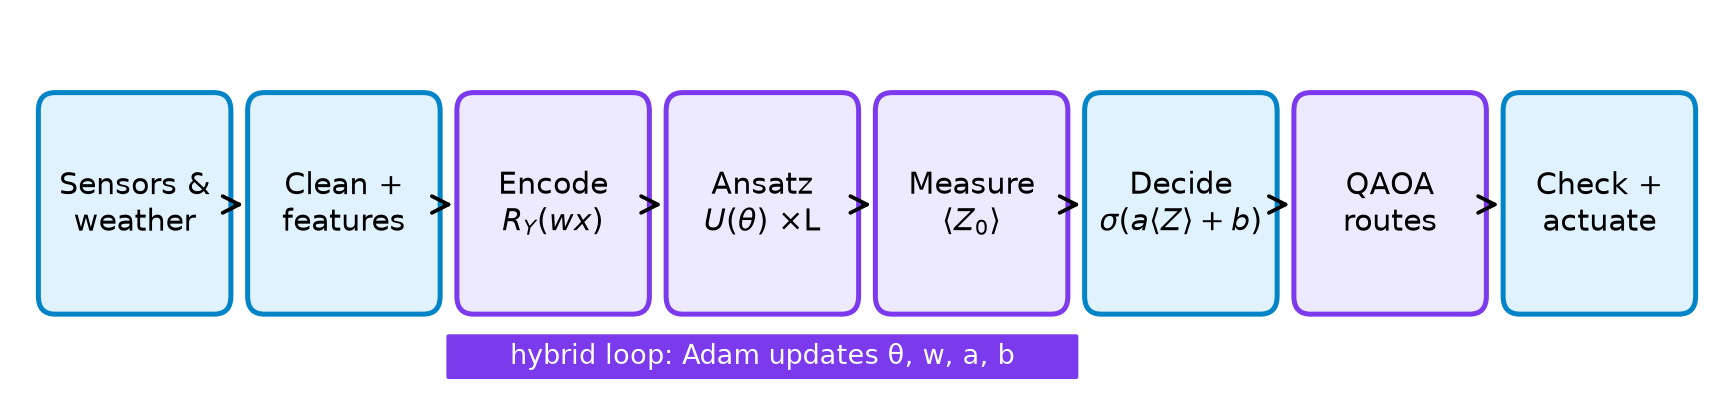
\includegraphics[width=0.92\textwidth]{pipeline.png}
\caption{QuantumITS pipeline. Blue: classical stages; purple: quantum or hybrid stages. Only encoding, the variational model, measurement and the QAOA sampler run on quantum hardware. Decisions, feasibility checks and actuation stay classical for safety.}
\label{fig:pipeline}
\end{figure*}

%=====================================================================
\section{Related Work}
\textbf{Variational classifiers and feature maps.} Havl\'{i}\v{c}ek \emph{et al.}~\cite{havlicek2019supervised} introduced Pauli-$ZZ$ feature maps for quantum kernels and variational classifiers. Schuld \emph{et al.}~\cite{schuld2020circuit} proposed circuit-centric classifiers. P\'{e}rez-Salinas \emph{et al.}~\cite{perez2020reuploading} showed that re-uploading data in several layers makes even one qubit a universal classifier. Schuld \emph{et al.}~\cite{schuld2021effect} explained why: a VQC computes a Fourier series whose frequencies are set by the encoding, so repeated or rescaled encodings add frequencies. Quantum kernels are sensitive to their bandwidth~\cite{shaydulin2022bandwidth}, and deep random circuits suffer from barren plateaus~\cite{mcclean2018barren}.

\textbf{Quantum optimisation for traffic.} Neukart \emph{et al.}~\cite{neukart2017traffic} formulated route assignment as a QUBO on a quantum annealer. Ising formulations of many combinatorial problems are given in~\cite{lucas2014ising}, and QAOA's behaviour and parameter strategies are analysed in~\cite{zhou2020qaoa}.

\textbf{Classical traffic prediction.} Deep learning is the classical state of the art for traffic-flow prediction~\cite{lv2015traffic}, which is why we compare against strong classical baselines on identical inputs.

\textbf{Error correction and mitigation.} Shor's code~\cite{shor1995scheme} was the first code to correct an arbitrary single-qubit error~\cite{nielsen2010qcqi}. Error-mitigation methods~\cite{temme2017mitigation} trade extra circuit runs for lower bias on near-term devices.

%=====================================================================
\section{Data and Problem Formulation}
\subsection{Dataset}
We use the Metro Interstate Traffic Volume dataset~\cite{hogue2019metro} (UCI \#492, also on Kaggle). It contains 48{,}204 hourly records (2012--2018) of westbound I-94 volume between Minneapolis and St~Paul together with weather-station readings. A real ITS would receive this kind of feed from each corridor. We removed sensor faults (a 9831~mm/h rain value and 0~K temperatures) and duplicate hours, which leaves \Nrows{} records. The binary target is \emph{congested} if the volume exceeds \Thr{}~veh/h, the median of the training years.

\subsection{Features and encoding choices}
We use four features so that each fits on one qubit: $x=[x_1,x_2,x_3,x_4]$ = (hour, weekend/holiday flag, temperature, weather severity 0--4). Weather severity maps \emph{Clear} to 0 and \emph{Snow/Thunderstorm} to 4. Preprocessing is classical and turns each reading into a rotation angle:
\begin{equation}
x_1=\tfrac{2\pi h}{24},\quad x_2=\pi\,\mathbb{1}[\text{weekend}],\quad x_3,x_4\in[0,\pi].
\label{eq:angles}
\end{equation}
Because $R_Y(2\pi)=-I$ is a global phase, the hour encoding is \emph{periodic}: 23:00 and 00:00 map to nearby states without an extra qubit. The binary flag becomes $\ket{0}$ or $\ket{1}$, which amounts to basis encoding on that qubit. Amplitude encoding would need only 2 qubits but loses absolute scale and needs a deep state-preparation circuit, so we chose angle encoding.

\subsection{Leakage-free evaluation}
Hourly traffic is a time series, so a random split leaks neighbouring hours. We train on 2012--2016 (\Npool{} records) and test on 2017--2018 (\Ntest{} records; \Nused{} sampled for evaluation, 53\% congested). Training subsets are class-balanced and drawn per seed. Every model sees the same samples.

\begin{table}[t]
\caption{Conceptual QML symbols interpreted for the ITS}
\label{tab:symbols}
\centering
\footnotesize
\begin{tabular}{@{}p{2.25cm}p{5.85cm}@{}}
\toprule
Symbol & Meaning in this case study \\
\midrule
$x=[x_1..x_4]$ & one junction snapshot: hour, day type, temperature, weather \\
$\ket{\psi(x)}=U_{\rm enc}(x)\ket{0000}$ & readings loaded as $R_Y$ rotations; a product state (no correlation yet) \\
$U_\phi(x)=e^{-i\phi(x)H}$ & feature map; $H=Z_kZ_l$ selects the coupled pair \\
$\phi_{kl}(x)$ & $(\pi-x_k)(\pi-x_l)$: joint effect, e.g.\ rush hour $\times$ snow \\
$\ket{\phi(x)}=U_\phi\ket{\psi}$ & entangled, data-dependent representation \\
$U(\theta)$ & trainable $R_ZR_YR_Z$ rotations and ring CNOTs \\
measurement & $\langle Z_0\rangle$ estimated from shots \\
classical decision & $\sigma(a\langle Z_0\rangle+b)>0.5$ $\Rightarrow$ re-time signals, advise routes \\
\bottomrule
\end{tabular}
\end{table}

%=====================================================================
\section{Method}
\subsection{Data re-uploading VQC}
Each of $L$ layers applies encoding with trainable input scaling, then a trainable block (Fig.~\ref{fig:circuit}):
\begin{equation}
\ket{\Phi(x;\Theta)}=\prod_{l=1}^{L}\Big[U(\theta_l)\bigotimes_{k=1}^{4}R_Y(w_{lk}x_k)\Big]\ket{0000},
\end{equation}
where $U(\theta_l)=\mathrm{CNOT}_{\rm ring}\bigotimes_k R_Z R_Y R_Z(\theta_{lk})$ and the ring couples $(1,2),(2,3),(3,4),(4,1)$. The measured $\langle Z_0\rangle$ enters a two-parameter classical head,
\begin{equation}
P(\text{congested}\mid x)=\sigma\big(a\,\langle\Phi|Z_0|\Phi\rangle+b\big).
\end{equation}
With $L{=}3$ the model has \nparams{} parameters, \ncx{} CNOTs and depth \depth{}. All parameters are trained jointly by full-batch Adam~\cite{kingma2015adam} on binary cross-entropy (150 steps, learning rate 0.05). Gradients are exact; on hardware they would come from parameter shifts. Re-uploading with scaling $w$ widens the Fourier spectrum the model can represent~\cite{schuld2021effect}.

\textbf{Feature map variant.} For the ablations we optionally insert the second-order map $U_\phi(x)=\prod_{(k,l)}\exp[-i(\pi-x_k)(\pi-x_l)Z_kZ_l]$ after each encoding. In gate form this is $R_{ZZ}(2\phi_{kl})$, i.e.\ CNOT--$R_Z$--CNOT.

\textbf{Baselines.} The \emph{standard VQC} encodes once, then applies two $R_YR_Z$ layers with linear CNOTs (26 parameters). It mirrors the textbook design. The \emph{quantum-kernel SVM} uses the fidelity kernel $K(x,x')=|\braket{\phi(bx)|\phi(bx')}|^2$ of a 2-repetition ZZ map, with bandwidth $b\in\{0.1,0.25,0.5,1\}$ and $C$ chosen by 3-fold cross-validation~\cite{shaydulin2022bandwidth}. Classical baselines are logistic regression, an RBF-SVM, a 200-tree random forest and a 16--16 MLP. They receive the hour as $(\sin,\cos)$ so that they are not disadvantaged.

\textbf{Simulation.} Circuits run on an exact batched statevector simulator written in PyTorch. It matches Qiskit~\cite{qiskit2024} to within $\simdiff$ on random parameters. Noisy runs use Qiskit Aer.

\begin{figure}[t]
\centering
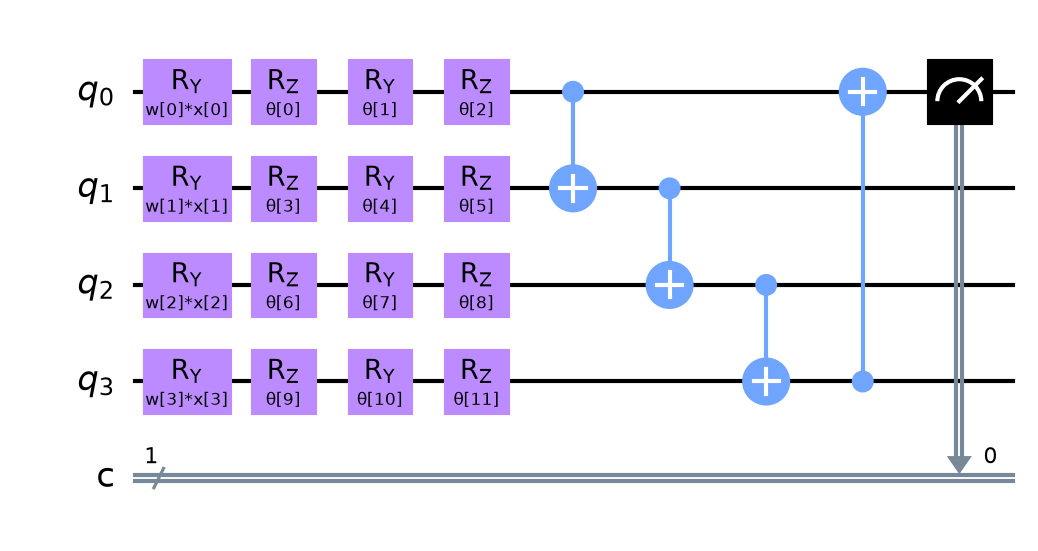
\includegraphics[width=\columnwidth]{circuit.png}
\caption{One re-uploading layer (repeated $L{=}3$ times). $R_Y(x_k w_k)$: feature-dependent encoding gates; $R_Z,R_Y,R_Z(\theta)$: trainable; CNOT ring: entanglement; final measurement of $q_0$.}
\label{fig:circuit}
\end{figure}

\subsection{Alternate-route recommendation as a QUBO}
$N{=}8$ traffic streams with demands $d_i$ approach the city. $x_i{=}1$ diverts stream $i$ to the alternate road. Delay on each road grows with the square of its load, a quadratic simplification of the BPR curve~\cite{bpr1964}:
\begin{equation}
J(x)=\frac{(D-d^\top x)^2}{C_{\rm m}}+\frac{(d^\top x)^2}{C_{\rm a}}+\tau\, d^\top x+P\,x_e .
\label{eq:qubo}
\end{equation}
Here $D=\sum_i d_i$ (loads are normalised), $C_{\rm m}{=}0.55$ and $C_{\rm a}{=}0.35$ are road capacities, $\tau{=}0.15$ is the detour cost, and the penalty $P{=}2$ keeps the emergency-vehicle stream $e$ on the cleared main road. Expanding (\ref{eq:qubo}) gives $J=x^\top Qx+c$ because $x_i^2=x_i$. Substituting $x_i=(1-Z_i)/2$ yields the Ising cost Hamiltonian $H_C=\sum_i h_iZ_i+\sum_{i<j}J_{ij}Z_iZ_j$~\cite{lucas2014ising}. We verified both forms against the direct cost on all 256 plans (max.\ error $\qubodiff$). Demands are drawn from real rush-hour I-94 volumes, giving 30 instances.

QAOA prepares $\ket{\gamma,\beta}=\prod_{j=1}^{p}e^{-i\beta_j\sum X_i}e^{-i\gamma_j H_C}\ket{+}^{\otimes N}$. COBYLA minimises $\langle H_C\rangle$ from a linear-ramp start plus two random restarts~\cite{zhou2020qaoa}. With costs normalised to $[0,1]$ we report the approximation ratio $r=1-\langle \tilde H_C\rangle$. The best of 128 sampled plans is passed to a classical feasibility check before release.

\subsection{Noise, mitigation and error correction}
We run the trained VQC on Qiskit Aer with depolarising errors $p_2$ on CNOTs and $p_2/10$ on single-qubit gates. Depolarising noise shrinks $\langle Z_0\rangle$ by an approximately constant factor $f$. We estimate $f$ by least squares on 100 training snapshots and divide it out before the decision (\emph{rescaling}). For error correction we protect a qubit that carries an encoded traffic reading with the 3-qubit bit-flip and phase-flip codes and with Shor's 9-qubit code~\cite{shor1995scheme,nielsen2010qcqi}. Correction is coherent, using CNOTs and Toffolis. Each physical qubit suffers $X$, $Y$ or $Z$ with probability $p/3$ each. A residual logical $X$, $Y$ or $Z$ is revealed by exactly two of the test states $\ket{0},\ket{+},\ket{+i}$, so the logical error rate is $p_L=\tfrac12(f_0+f_++f_{+i})$, where $f$ is each test's failure rate.

%=====================================================================
\section{Results}
\subsection{Congestion prediction}
Table~\ref{tab:main} and Fig.~\ref{fig:lc} report mean test performance over three seeds. With 1000 training snapshots the re-uploading VQC reaches \accOursM{} accuracy and \aucOurs{} AUC, level with the RBF-SVM (\accSVMM{}), random forest (\accRFM{}) and MLP (\accMLPM{}). The textbook single-encoding VQC reaches \accStdM{}. The quantum-kernel SVM is weakest (\accQKM{}) even after bandwidth tuning. Our earlier coursework VQC (Exp.~5: temperature, rain, clouds and hour, random split) reached only about 0.66. The gain comes from feature selection, chiefly a weekend/holiday qubit, and from re-uploading, not from more qubits. At $n{=}50$ the VQC is less stable across seeds (\accOursFifty{}), and it overtakes the standard VQC once $n\ge 250$.

\begin{table}[t]
\caption{Test performance on 2017--18 (mean of 3 seeds, $n{=}1000$)}
\label{tab:main}
\centering
\footnotesize
\begin{tabular}{@{}lccccc@{}}
\toprule
Model & Acc. & $\pm$sd & AUC & Recall & Fit (s) \\
\midrule
\textbf{Re-uploading VQC (ours)} & \textbf{\accOursM} & \sdOursM & \aucOurs & \recOurs & \fitOurs \\
Standard VQC & \accStdM & \sdStdM & \aucStd & \recStd & \fitStd \\
Quantum-kernel SVM & \accQKM & \sdQKM & \aucQK & \recQK & \fitQK \\
\midrule
Logistic regression & \accLRM & \sdLRM & \aucLR & \recLR & \fitLR \\
SVM (RBF) & \accSVMM & \sdSVMM & \aucSVM & \recSVM & \fitSVM \\
Random forest & \accRFM & \sdRFM & \aucRF & \recRF & \fitRF \\
MLP (16-16) & \accMLPM & \sdMLPM & \aucMLP & \recMLP & \fitMLP \\
\bottomrule
\end{tabular}
\end{table}

\begin{figure}[t]
\centering
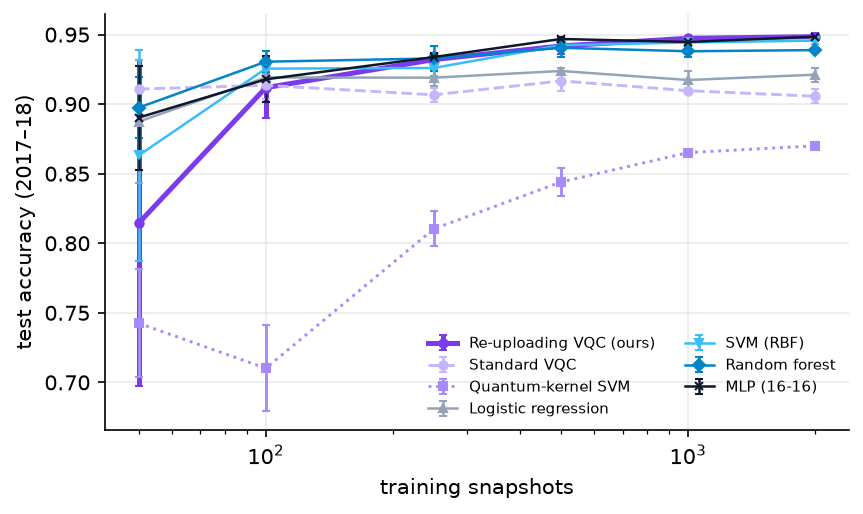
\includegraphics[width=\columnwidth]{learning_curve.png}
\caption{Test accuracy vs.\ training-set size (mean $\pm$ sd, 3 seeds). Purple: quantum; blue/grey: classical.}
\label{fig:lc}
\end{figure}

\subsection{Ablation: what makes the VQC work?}
Fig.~\ref{fig:ablation} varies one design choice at a time ($n{=}500$). Re-uploading is essential. With a single layer and one trainable block the model cannot fit the data (\ablG{} at $L{=}1$), while two or more layers reach the plateau ($L{=}2$: \ablH, $L{=}3$: \ablC, $L{=}5$: \ablJ). Removing trainable input scaling costs accuracy (\ablD). Ring and linear entanglement perform similarly (\ablE). Adding the ZZ feature map \emph{hurts}, both in the standard VQC (\ablA$\to$\ablB) and in ours (\ablF). Its products $(\pi-x_k)(\pi-x_l)$ inject large, rapidly varying phases that the small ansatz cannot exploit. This matches our Exp.~2/5 coursework findings and the bandwidth argument of~\cite{shaydulin2022bandwidth}. Non-cyclic hour encoding ($\pi h/24$) gives \ablK, which is indistinguishable from the cyclic version. Midnight hours are almost all free-flowing, so the wrap-around rarely matters for this label. The periodic map costs nothing, though, and is safer for targets that peak near midnight.

\begin{figure}[t]
\centering
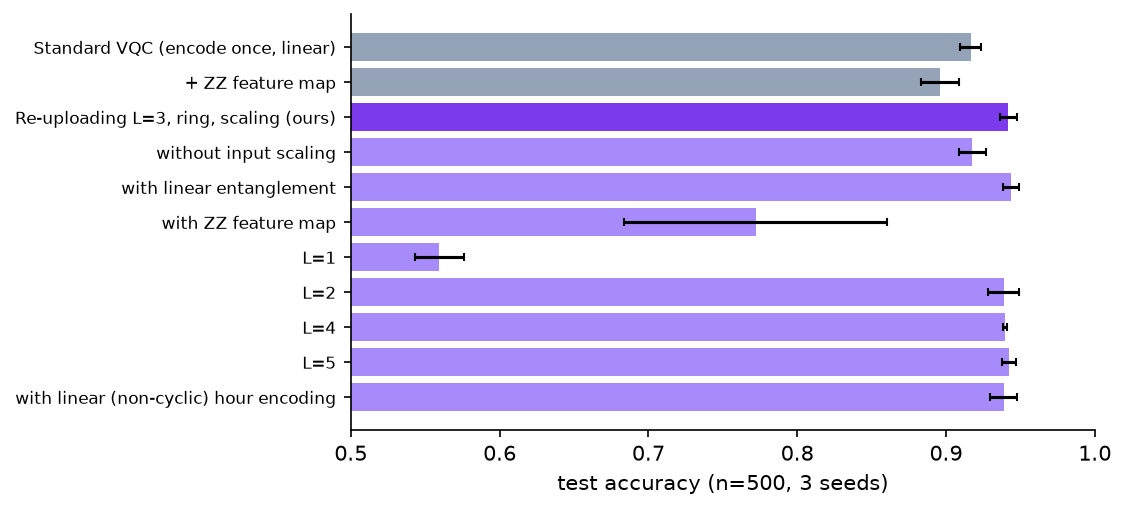
\includegraphics[width=\columnwidth]{ablation.png}
\caption{Ablation of VQC design choices ($n{=}500$, mean $\pm$ sd).}
\label{fig:ablation}
\end{figure}

\subsection{Hardware noise and shot budget}
Fig.~\ref{fig:noise} shows that the classifier degrades gracefully. Accuracy is \noiseIdeal{} with exact noiseless probabilities, \noiseRawB{} at $p_2{=}1\%$ and \noiseRawD{} at $p_2{=}5\%$ with 1024 shots (differences below about 1\% are within shot noise), even though depolarising noise shrinks $\langle Z_0\rangle$ by $f{=}\shrinkB$ and $f{=}\shrinkD$ respectively. Accuracy survives because the learned bias $b$ is small: the decision boundary sits near $\langle Z_0\rangle\approx0$, and a uniform shrink does not move it. The \emph{probabilities} reported to operators are, however, pulled towards 0.5. The mean deviation from the noiseless probability at $p_2{=}5\%$ is \probErrRawD, and dividing by the calibrated $f$ reduces it to \probErrMitD{} (Fig.~\ref{fig:noise}, right). Accuracy needs only a modest number of shots: 16 shots give \shotsSixteen{} and 1024 shots give \shotsK.

\begin{figure*}[t]
\centering
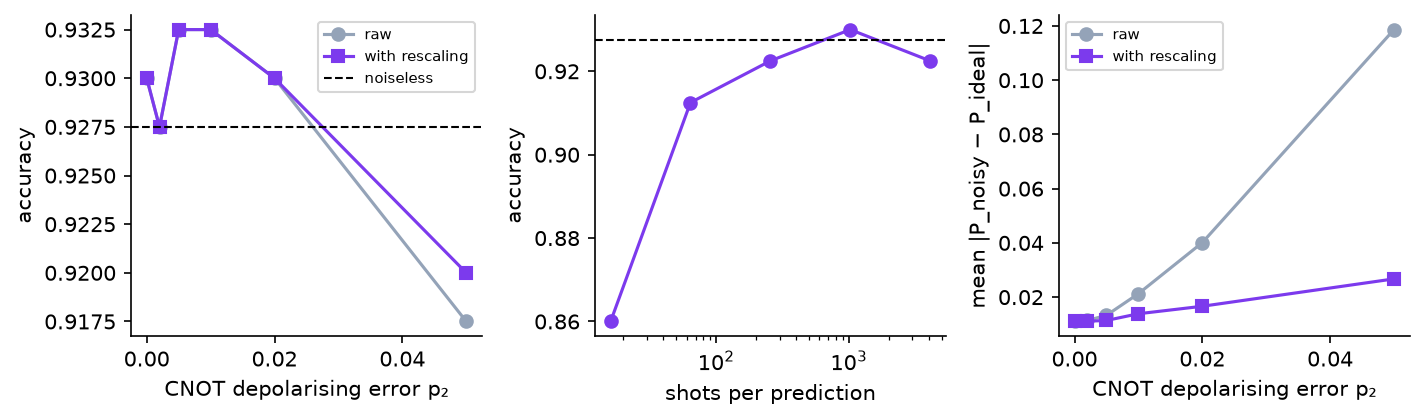
\includegraphics[width=0.85\textwidth]{noise.png}
\caption{Left: accuracy under depolarising noise. Middle: accuracy vs.\ shots (noiseless). Right: mean error of the predicted probability, raw and with the one-parameter rescaling.}
\label{fig:noise}
\end{figure*}

\subsection{Latency against the one-second budget}
Table~\ref{tab:latency} lists the median single-snapshot latency. Every model, including Aer with 1024 shots (\latAer{}~ms), fits comfortably within 1000~ms on a laptop CPU. These are simulator timings. Cloud hardware adds queueing and network round-trips of seconds to minutes, which currently rules out on-line use on real devices.

\begin{table}[t]
\caption{Median (p95) latency per snapshot, ms}
\label{tab:latency}
\centering
\footnotesize
\begin{tabular}{@{}lcc@{}}
\toprule
Stage & median & p95 \\
\midrule
Preprocessing (classical) & \latPre & \latpPre \\
VQC, exact simulator & \latVqc & \latpVqc \\
VQC, Aer, 1024 shots & \latAer & \latpAer \\
Quantum-kernel SVM & \latQk & \latpQk \\
Random forest & \latRf & \latpRf \\
MLP & \latMlp & \latpMlp \\
\bottomrule
\end{tabular}
\end{table}

\subsection{Route optimisation with QAOA}
Over 30 real-demand instances (Table~\ref{tab:qaoa}, Fig.~\ref{fig:qaoa}), QAOA raises the approximation ratio from \arR{} (uniform sampling) to \arOne{} at $p{=}1$ and \arFour{} at $p{=}4$. The probability of a plan within 2\% of the optimum rises from \pnearR\% to \pnearFour\%. In every instance the best of 128 samples was the exact optimum (mean gap \gapFour\%), but at $N{=}8$ even 128 uniform samples would very likely contain a near-optimal plan. Exact enumeration of the $2^8$ plans takes \msEx{}~ms, while QAOA parameter training takes \msOne--\msFour{}~ms in simulation. At this size QAOA has no practical advantage. Its value is as a hybrid template that would apply to larger regional sub-problems where exhaustive search is impossible.

\begin{table}[t]
\caption{Route optimisation over 30 instances (mean)}
\label{tab:qaoa}
\centering
\footnotesize
\begin{tabular}{@{}lcccc@{}}
\toprule
Method & $\langle r\rangle$ & $P_{\le2\%}$ (\%) & best gap (\%) & time (ms) \\
\midrule
Random sampling & \arR & \pnearR & -- & -- \\
QAOA $p{=}1$ & \arOne & \pnearOne & \gapOne & \msOne \\
QAOA $p{=}2$ & \arTwo & \pnearTwo & \gapTwo & \msTwo \\
QAOA $p{=}3$ & \arThree & \pnearThree & \gapThree & \msThree \\
QAOA $p{=}4$ & \arFour & \pnearFour & \gapFour & \msFour \\
\midrule
Exact enumeration & 1 & -- & \gapEx & \msEx \\
Greedy & -- & -- & \gapGr & \msGr \\
Simulated annealing & -- & -- & \gapSa & \msSa \\
\bottomrule
\end{tabular}
\end{table}

\begin{figure}[t]
\centering
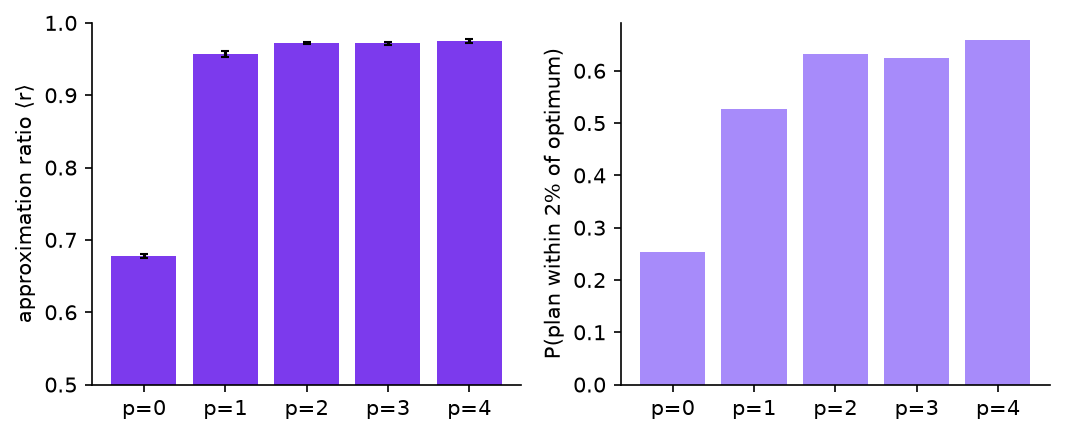
\includegraphics[width=\columnwidth]{qaoa.png}
\caption{QAOA approximation ratio and probability of near-optimal plans vs.\ depth ($p{=}0$: uniform sampling).}
\label{fig:qaoa}
\end{figure}

\subsection{Error-protected quantum output}
Fig.~\ref{fig:qec} shows the logical error rate under depolarising noise. Each 3-qubit code lets one error type through while exposing three qubits, so both are \emph{worse} than no protection (at $p{=}1\%$: \qecBB{} vs.\ \qecUB). Shor's code corrects every single-qubit error, giving $p_L\propto p^2$ and \qecSB{} at $p{=}1\%$, i.e.\ \shorGain$\times$ fewer errors. Above roughly $p\approx 8\%$ (its pseudo-threshold under this noise model) it loses to the bare qubit. The price is 9 physical qubits per logical qubit: 36 for our VQC and 72 for the 8-stream QAOA, before repeated syndrome rounds.

\begin{figure}[t]
\centering
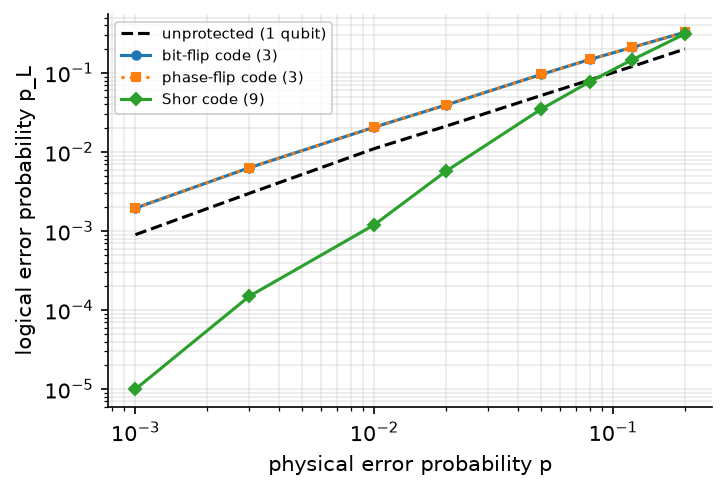
\includegraphics[width=0.85\columnwidth]{qec.png}
\caption{Logical vs.\ physical error rate under depolarising noise (Qiskit Aer, 20k shots per point).}
\label{fig:qec}
\end{figure}

%=====================================================================
\section{Discussion}
\textbf{What should be quantum?} Sensor ingestion, cleaning, feature engineering, thresholds, feasibility checks and actuation must remain classical, because they are safety-critical and need deterministic, auditable behaviour. The quantum candidates are the pattern-recognition model and the combinatorial sampler. Our results show that a carefully encoded 4-qubit VQC can \emph{match}, but not beat, classical models on this low-dimensional task. QAOA likewise produces good but not better route plans at 8 variables. Following~\cite{bowles2024better}, we treat this parity as the honest outcome of a fair comparison, not as a failure.

\textbf{Design lessons.} (i) Feature and encoding choices come first: a single basis-encoded day-type qubit carries most of the signal, and a periodic hour angle is free. (ii) Re-uploading with trainable scaling beats adding entangling feature maps. (iii) Depolarising noise mainly miscalibrates probabilities rather than flipping decisions, and a single calibrated rescaling largely repairs it. (iv) Error correction must match the noise. Only a code that handles $X$, $Y$ and $Z$ helps under depolarising noise, at a 9$\times$ qubit cost.

\textbf{Limitations.} All results come from simulators. Our route model is a stylised two-road network. The data come from a single corridor, and the binary target is coarse. Hardware queueing latency, readout error and fault-tolerant overheads are not measured.

%=====================================================================
\section{Conclusion}
QuantumITS is an end-to-end, reproducible hybrid pipeline for a national ITS. A data re-uploading VQC predicted congestion on real 2017--18 traffic with \accOursM{} accuracy, on par with the best classical baselines and far above a textbook VQC. QAOA solved a congestion-aware QUBO for alternate routing, and Shor's code was the only option that protected a quantum output under realistic noise. Quantum components should for now be deployed as benchmarked modules behind classical decision and safety layers. Future work will test real hardware, graph-structured multi-junction inputs on more qubits, and regional QAOA sub-problems with 50+ variables.

\begin{thebibliography}{00}
\bibitem{preskill2018nisq} J. Preskill, ``Quantum computing in the NISQ era and beyond,'' \emph{Quantum}, vol. 2, p. 79, 2018.
\bibitem{biamonte2017qml} J. Biamonte, P. Wittek, N. Pancotti, P. Rebentrost, N. Wiebe, and S. Lloyd, ``Quantum machine learning,'' \emph{Nature}, vol. 549, pp. 195--202, 2017.
\bibitem{cerezo2021vqa} M. Cerezo \emph{et al.}, ``Variational quantum algorithms,'' \emph{Nature Reviews Physics}, vol. 3, pp. 625--644, 2021.
\bibitem{bowles2024better} J. Bowles, S. Ahmed, and M. Schuld, ``Better than classical? The subtle art of benchmarking quantum machine learning models,'' arXiv:2403.07059, 2024.
\bibitem{havlicek2019supervised} V. Havl\'{i}\v{c}ek \emph{et al.}, ``Supervised learning with quantum-enhanced feature spaces,'' \emph{Nature}, vol. 567, pp. 209--212, 2019.
\bibitem{schuld2020circuit} M. Schuld, A. Bocharov, K. M. Svore, and N. Wiebe, ``Circuit-centric quantum classifiers,'' \emph{Phys. Rev. A}, vol. 101, 032308, 2020.
\bibitem{perez2020reuploading} A. P\'{e}rez-Salinas, A. Cervera-Lierta, E. Gil-Fuster, and J. I. Latorre, ``Data re-uploading for a universal quantum classifier,'' \emph{Quantum}, vol. 4, p. 226, 2020.
\bibitem{schuld2021effect} M. Schuld, R. Sweke, and J. J. Meyer, ``Effect of data encoding on the expressive power of variational quantum-machine-learning models,'' \emph{Phys. Rev. A}, vol. 103, 032430, 2021.
\bibitem{shaydulin2022bandwidth} R. Shaydulin and S. M. Wild, ``Importance of kernel bandwidth in quantum machine learning,'' \emph{Phys. Rev. A}, vol. 106, 042407, 2022.
\bibitem{mcclean2018barren} J. R. McClean, S. Boixo, V. N. Smelyanskiy, R. Babbush, and H. Neven, ``Barren plateaus in quantum neural network training landscapes,'' \emph{Nature Communications}, vol. 9, 4812, 2018.
\bibitem{farhi2014qaoa} E. Farhi, J. Goldstone, and S. Gutmann, ``A quantum approximate optimization algorithm,'' arXiv:1411.4028, 2014.
\bibitem{lucas2014ising} A. Lucas, ``Ising formulations of many NP problems,'' \emph{Frontiers in Physics}, vol. 2, p. 5, 2014.
\bibitem{zhou2020qaoa} L. Zhou, S.-T. Wang, S. Choi, H. Pichler, and M. D. Lukin, ``Quantum approximate optimization algorithm: Performance, mechanism, and implementation on near-term devices,'' \emph{Phys. Rev. X}, vol. 10, 021067, 2020.
\bibitem{neukart2017traffic} F. Neukart, G. Compostella, C. Seidel, D. von Dollen, S. Yarkoni, and B. Parney, ``Traffic flow optimization using a quantum annealer,'' \emph{Frontiers in ICT}, vol. 4, p. 29, 2017.
\bibitem{lv2015traffic} Y. Lv, Y. Duan, W. Kang, Z. Li, and F.-Y. Wang, ``Traffic flow prediction with big data: A deep learning approach,'' \emph{IEEE Trans. Intelligent Transportation Systems}, vol. 16, no. 2, pp. 865--873, 2015.
\bibitem{shor1995scheme} P. W. Shor, ``Scheme for reducing decoherence in quantum computer memory,'' \emph{Phys. Rev. A}, vol. 52, R2493, 1995.
\bibitem{nielsen2010qcqi} M. A. Nielsen and I. L. Chuang, \emph{Quantum Computation and Quantum Information}, 10th anniv. ed. Cambridge Univ. Press, 2010.
\bibitem{temme2017mitigation} K. Temme, S. Bravyi, and J. M. Gambetta, ``Error mitigation for short-depth quantum circuits,'' \emph{Phys. Rev. Lett.}, vol. 119, 180509, 2017.
\bibitem{hogue2019metro} J. Hogue, ``Metro Interstate Traffic Volume,'' UCI Machine Learning Repository, 2019, doi: 10.24432/C5X60B.
\bibitem{kingma2015adam} D. P. Kingma and J. Ba, ``Adam: A method for stochastic optimization,'' in \emph{Proc. ICLR}, 2015.
\bibitem{bpr1964} Bureau of Public Roads, \emph{Traffic Assignment Manual}. U.S. Dept. of Commerce, 1964.
\bibitem{qiskit2024} A. Javadi-Abhari \emph{et al.}, ``Quantum computing with Qiskit,'' arXiv:2405.08810, 2024.
\end{thebibliography}

\end{document}
